\section{汽车产品零件BOM表}
点击主页\underline{产品BOM表},即可进入BOM表主页,如图\ref{fig:PDM_index}。
\begin{figure}[H]
\centering

\includegraphics[width=0.9\linewidth]{figure/PDM_index}
\caption{产品BOM表主页}
\label{fig:PDM_index}
\end{figure}


本文的BOM表的设计,参考动态菜单的设计思路。汽车产品和零件信息的显示利用HTML中的\verb|ul和li|标签实现,信息的检索使用SQL查询等语句实现,相关代码参见附录。

为了事项动态BOM表的动态显示效果,本文利用JavaScript的封装JQeury实现编写代码实现。当用户点击``车型及其零件''前的$"+"/"-"$时,执行如图\ref{fig:BOM0}所示的算法。每当用户点击汽车产品名称前的$"+"/"-"$时,执行如图\ref{fig:BOM1}所示的算法。
\begin{figure}[H]
\centering
\subfigure[单击``车型及其零件''事件算法]{%
	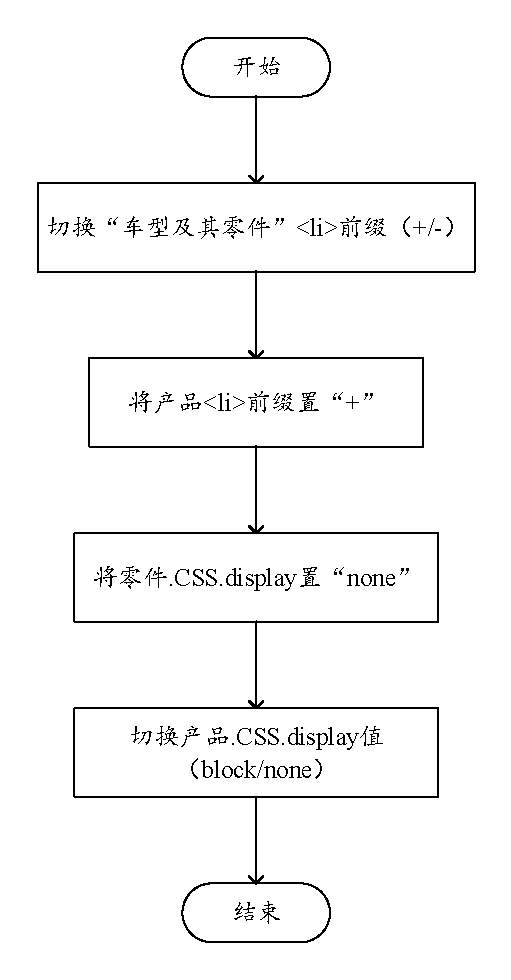
\includegraphics[width=0.4\linewidth]{figure/BOM0}
	\label{fig:BOM0}}
	\quad
\subfigure[单击产品事件算法]{%
	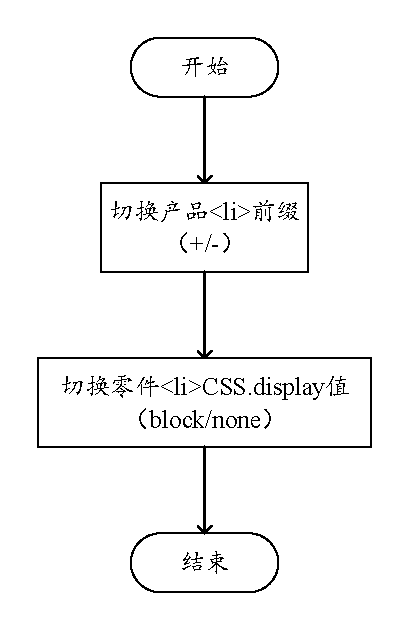
\includegraphics[width=0.4\linewidth]{figure/BOM}
	\label{fig:BOM1}}
\caption{BOM动态显示算法}
\label{fig:BOM}
\end{figure}

单击``车型及其零件''前的``+'',可以展开产品目录;单击汽车产品名称前的``+'',可以打开
产品的零件目录。目录展开后, 点击``$-$'' 可以收起目录。鼠标移到对应产品名或者零件,字体将变红,便于用户识别选择的对象,如图\ref{fig:BOM_spread}。
\begin{figure}[H]
\centering

\includegraphics[width=0.9\linewidth]{figure/BOM_spread}
\caption{BOM表显示图}
\label{fig:BOM_spread}
\end{figure}

BOM表中的产品名和零件名词都是超链接,单击产品(或零件)名称可连接到相关产品(或零件),例如单击\underline{帕萨特 2016款 280TSI DSG尊荣版},能得到汽车产品信息表单(如图\ref{fig:BOM_PROD}),如单击\underline{帕萨特汽车车门},能到零件信息表单(如图\ref{fig:BOM_PART})。在产品表单中,有``零件信息''、``修改''和``删除''链接;在零件表单中,有``修改''和``删除''链接。
\begin{figure}[H]
\centering

\includegraphics[width=0.9\linewidth]{figure/BOM_PROD}
\caption{BOM-产品表单}
\label{fig:BOM_PROD}
\end{figure}
\begin{figure}[H]
\centering

\includegraphics[width=0.9\linewidth]{figure/BOM_PART}
\caption{BOM-零件表单}
\label{fig:BOM_PART}
\end{figure}




